% -*-memoria.tex-*-
% Este fichero es parte de la plantilla LaTeX para
% la realización de Proyectos Final de Carrera, protejido
% bajo los términos de la licencia GFDL.
% Para más información, la licencia completa viene incluida en el
% fichero fdl-1.3.tex

% Copyright (C) 2009 Pablo Recio Quijano 

%-------------------------------------------------------
% ---- Plantilla para libros / memorias PFC -----

% Realizada por Pablo Recio Quijano y Noelia Sales Montes 
% Formato de portada y primera página tomado del PFC de
% Francisco Javier Vázquez Púa, en su proyecto 'libgann'
% -------------------------------------------------------

\documentclass[a4paper,11pt]{book}
%\usepackage{filecontents}
%\usepackage[style=authoryear,backend=bibtex]{biblatex}
% Necesario para poder hacer funcionar la bibliografia hecha en BibTeX

\usepackage{./estilos/estiloBase} % Basicamente son todas las
                                  % librerias usadas. En caso de que
                                  % falten librerias se van añadiendo
                                  % al fichero.
\usepackage{./estilos/colores}  % Algunos colores ya generados, para
                                % los algunos estilos más avanzados.
\usepackage{./estilos/comandos} % Algunos comandos personalizados

\graphicspath{{./imagenes/}} % Indicamos la ruta donde se encuentran
                             % las imagenes, para ahorrarnos la ruta
                             % completa, y solo modificar aquí si en
                             % un momento dado lo movemos


\begin{document}

% Renombramos las figuras y las tablas
\renewcommand{\figurename}{Figura}
\renewcommand{\listfigurename}{Indice de figuras}
\renewcommand{\tablename}{Tabla}
\renewcommand{\listtablename}{Indice de tablas}

\pagestyle{empty}
% -*-portada.tex-*-
% Este fichero es parte de la plantilla LaTeX para
% la realización de Proyectos Final de Carrera, protejido
% bajo los términos de la licencia GFDL.
% Para más información, la licencia completa viene incluida en el
% fichero fdl-1.3.tex

% Fuente tomada del PFC 'libgann' de Javier Vázquez Púa

\begin{titlepage}

  \begin{center}

    
\includegraphics[scale=0.2]{logo_uca.png} \\
    
    \vspace{2.0cm}
    
    \LARGE{\textbf{ESCUELA SUPERIOR DE INGENIERÍA}} \\
    
    \vspace{1.0cm}
    
    \Large{\textbf{INGENIERÍA TÉCNICA EN INFORMÁTICA DE SISTEMAS}} \\
    
    \vspace{3.0cm}
    
    \Large{LA AVENTURA DEL CÁDIZ DE 1812: VIDEOJUEGO REALIZADO EN UNITY PARA FINES LÚDICOS Y DIVULGATIVOS} \\
    
    \vspace{2.0cm}
    
    \Large{Alicia Guardeño Albertos} \\
  
    \vspace{0.5cm}

    \large{\today}
    
  \end{center}
\end{titlepage}

\cleardoublepage

% -*-primerahoja.tex-*-
% Este fichero es parte de la plantilla LaTeX para
% la realización de Proyectos Final de Carrera, protejido
% bajo los términos de la licencia GFDL.
% Para más información, la licencia completa viene incluida en el
% fichero fdl-1.3.tex

% Fuente tomada del PFC 'libgann' de Javier Vázquez Púa

\begin{center}

  
\includegraphics[scale=0.2]{logo_uca.png} \\

  \vspace{2.0cm}

  \Large{ESCUELA SUPERIOR DE INGENIERÍA} \\

  \vspace{1.0cm}

  \large{INGENIERO TÉCNICO EN INFORMÁTICA DE SISTEMAS} \\

  \vspace{2.0cm}

  \large{LA AVENTURA DEL CÁDIZ DE 1812: VIDEOJUEGO REALIZADO EN UNITY PARA FINES LÚDICOS Y DIVULGATIVOS} \\

  \vspace{1.0cm}

\end{center}

\begin{itemize}
\item \large{Departamento: Ingeniería Informática}
\item \large{Director del proyecto: Manuel Palomo Duarte}
\item \large{Autor del proyecto: Alicia Guardeño Albertos}
\end{itemize}

\vspace{1.0cm}

\begin{flushright}
  \large{Cádiz, \today} \\

  \vspace{2.5cm}

  \large{Fdo: Alicia Guardeño Albertos}
\end{flushright}

\cleardoublepage
\pagestyle{plain}

\frontmatter % Introducción, índices ...

% -*-previo.tex-*-
% Este fichero es parte de la plantilla LaTeX para
% la realización de Proyectos Final de Carrera, protejido
% bajo los términos de la licencia GFDL.
% Para más información, la licencia completa viene incluida en el
% fichero fdl-1.3.tex

% Copyright (C) 2009 Pablo Recio Quijano 

\section*{Agradecimientos}

Me gustaria agradecer y dedicar este texto a:
\begin{itemize}
\item Manuel Palomo por su labor de tutorización y consejos.
\item Javier Cadenas por su asesoramiento respecto al diseño de videojuegos orientado al género de las aventuras gráficas.
\item José Joaquín Rodríguez por sus consejos y sugerencias sobre cuales libros escoger para la documentación histórica.
\item Celia Fermoselle, \cursiva{boredBit}, Laura J. Torres, Daniel Brey y Encarnación M. R. porque sin su colaboración este proyecto no tendría la calidad que tiene. 
\item Eric Juste por ser mi querido \cursiva{betatester} y apoyo moral durante la realización del proyecto.
\item Toda mi familia por su cariño incondicional durante todo este tiempo.
\item La comunidad de Unity por ayudarme a resolver dudas y consejos sobre la implementación.
\item La comunidad de ZehnGames, Games Tribune y muchos más por su labor de difusión de mi proyecto, sin ella no habría conseguido a mis colaboradores.
\end{itemize}

\cleardoublepage

\section*{Licencia} % Por ejemplo GFDL, aunque puede ser cualquiera

Este documento ha sido liberado bajo Licencia GFDL 1.3 (GNU Free
Documentation License). Se incluyen los términos de la licencia en
inglés al final del mismo. Sin embargo, las imágenes de videojuegos comerciales incluidos están sujetos a copyright y no se distribuyen bajo licencia libre.\\

Copyright (c) 2014 Alicia Guardeño Albertos.\\

Permission is granted to copy, distribute and/or modify this document under the
terms of the GNU Free Documentation License, Version 1.3 or any later version
published by the Free Software Foundation; with no Invariant Sections, no
Front-Cover Texts, and no Back-Cover Texts. A copy of the license is included in
the section entitled "GNU Free Documentation License".\\

\cleardoublepage

\section*{Notación y formato}
Para poder mantener un estilo uniforme y legible, a lo largo de esta memoria de \textbf{Proyecto Final de Carrera} se ha utilizado la siguiente notación:
\begin{itemize}
\item Para referirnos a nombres de ficheros o funciones de un lenguaje usaremos: \comando{unity.cs}.
\item Cuando mencionemos el nombre de un programa se hará de la siguiente manera: \programa{Unity}.
\item Los nombres de los objetos de \programa{Unity3D} se escriben con este formato: \gameobject{GameController}.
\item Los componentes de los objetos, excepto cuando se traten de \emph{Scripts}, tendrán el siguiente formato: \gocomponent{Rigidbody}.
\item En el caso de adjuntar un fragmento de código, utilizamos bloques como el siguiente:
\end{itemize}

\lstinputlisting[style=C++]{./codigo/hola_mundo.cs}
\cleardoublepage

\tableofcontents
\listoffigures
\listoftables

\mainmatter % Contenido en si ...
%-------------------------------------------------
\setlength{\parskip}{\baselineskip} %Lo pongo aqui para evitar el salto de línea en los índices
%\setlength{\parskip}{0.5em}
%-------------------------------------------------

\chapter{Motivación y contexto del proyecto}
\label{chap:introduccion}
Este es el documento de diseño de \nombrejuego. El cual es un videojuego en 2D del género de las aventuras gráficas, con una ambientación en la Cádiz actual cuyo objetivo es tanto de entretener al jugador como que aprenda anécdotas y hechos relacionados con Cádiz en los años que fue asediada y vieron nacer la Constitución de 1812.

    \section{Concepto del videojuego}
        \nombrejuego es un videojuego en el que controlaremos a un estudiante de la Licenciatura de Historia de la Universidad de Cádiz, que recientemente ha suspendido un examen y va al despacho a pedir una revisión para su nota. Sin embargo, no logra encontrar al profesor y se embarcará en una aventura para descubrir el paradero de dicho profesor ayudándose de las pistas obtenidas al resolver puzzles, teniendo estos siempre una relación con la Cádiz de 1812. El videojuego tiene que estar completamente documentado, pues una gran gran parte de la jugabilidad y de la parte educativa del juego, recae completamente en el buen diseño que se haga de los puzzles, estancias e interacciones con otros personajes no controlables.
        
    \section{Género}
        \nombrejuego pretende seguir el patrón de las aventuras gráficas antiguas. Dicho género basa sus mecánicas en ir avanzando por el mundo, escenario o juego a través de la resolución de diversos puzzles, planteados como situaciones que se suceden en la historia, interactuando con personajes y objetos a través de un menú de acciones o interfaz similar, utilizando un cursor para manejar al personaje y realizar las distintas acciones.
        
    \section{Propósito y público objetivo}
        El principal objetivo de \nombrejuego es de proporcionar documentación en español sobre el diseño de videojuegos, y más específicamente en el campo de las aventuras gráficas con el documento de diseño de puzzles. También el de promocionar la historia de Cádiz. Finalmente, realizar el videojuego a partir de los diseños, poniendo a disposición de la gente el código documentado del juego y así promocionar el desarrollo organizado para proyectos con una mediana envergadura. No obstante, debe de ser un producto que sea jugable y ameno para que este desarrollo haya cumplido con sus objetivos.
        
        \nombrejuego está dirigido a todas las edades a partir de los seis años, pero principalmente a los jóvenes por ser un videojuego sencillo y tratado con un humor más juvenil. 
        
    \section{Resumen del flujo de juego}%Game flow summary
        Si bien el videojuego va a ser 2D, el movimiento del personaje dentro de los escenarios (dentro de las zonas donde se pueda caminar) será de arriba y abajo, derecha e izquierda y en diagonales. Luego para moverse entre los escenarios, se hará uso de un mapa con las localizaciones marcadas. Para poder avanzar en el juego será necesario resolver puzzles en los escenarios para poder acceder a nuevas localizaciones en el mapa.
        
    \section{Estilo visual}
    \nombrejuego tendrá un estilo sencillo, sin ser demasiado detallista para encajar con su carácter amigable y accesible. El estilo visual que más encaja sería el de las aventuras gráficas antiguas, las cuales eran gráficos pixelados asemejando a dibujos animados o cómics. Los personajes y escenarios serán caricaturescos, con colores vivos y trazos simples. En el caso de los escenarios, estos estarán basados en sitios reales a los que se les habrá simplificado o modificado para encajar con el estilo visual del videojuego.
        
    \section{Alcance del proyecto}%Project scope
    El objetivo principal es desarrollar un sistema de juego sólido, al que podamos ir añadiéndole contenidos sin apenas dificultad. En primera instancia el juego contará con nueve escenarios distintos, cada uno con uno o dos puzzles. Cada escenario representará un lugar distinto de Cádiz, y por consiguiente con una temática distinta tanto visualmente como en el problema histórico a tratar en el puzzle.
    
        \subsection{Número de niveles}
        En un principio son nueve niveles, pero este número puede variar con facilidad.
        
        \subsection{Número de Personajes No Jugables (PNJ o NPC en inglés)}
        Por ahora el número de PNJs definidos son unos cinco.
        
        \subsection{Número de puzzles}
        En un principio son diez puzzles, incluyendo un puzzle final que haga un repaso de todos las anécdotas históricas relatadas en el videojuego.


\chapter{Organización temporal}
\label{chap:planificacion}



En este capítulo se expone la planificación de tareas que se ha seguido para desarrollar \nombrejuego{}. En primer lugar se adjunta el diagrama de Gantt completo para, más adelante, complementarlo con un breve comentario de cada tarea.

\section{Diagrama de Gantt}
Como puede observarse en el diagrama de Gantt, en el apartado artístico de \nombrejuego{} participan más personas. Esto se debe a que no poseía ni poseo los conocimientos o destrezas requeridos para crear modelos 2D y sus animaciones, escenarios de la ciudad de Cádiz, todo en \cursiva{pixel art}, piezas musicales, efectos de sonido ni un guión de diálogos y descripciones completo con su correspondiente traducción al inglés. Por ello, he contactado con gente con experiencia en dichas materias dispuestos a colaborar en el desarrollo de un videojuego completamente libre. Además de una persona que asesore en el área histórica del videojuego para evitar incongruencias. Finalmente, los participantes adicionales son:

\begin{itemize}
\item Celia Fermoselle: artista especializada en\cursiva{pixel art} encargada de diseñar, dibujar, animar a los personajes, objetos y escenarios del juego.
\item boredBit: grupo formado por Dmitry Jbanov y Manu Garrido que se encargan de componer y producir la banda sonora completa y efectos de sonido para el juego.
\item Daniel Brey: encargado de escribir en su mayoría del guión de diálogos y descripciones del juego.
\item Laura J. Torres: encargada en traducir el guión del juego del español al inglés.
\item Encarnación M. R. : encargada en asesorar el contenido histórico del proyecto para evitar incongruencias.
\end{itemize}

El diagrama de Gantt sobre la planificación del proyecto es el siguiente:

\begin{figure}[H] 
  \begin{center}
    %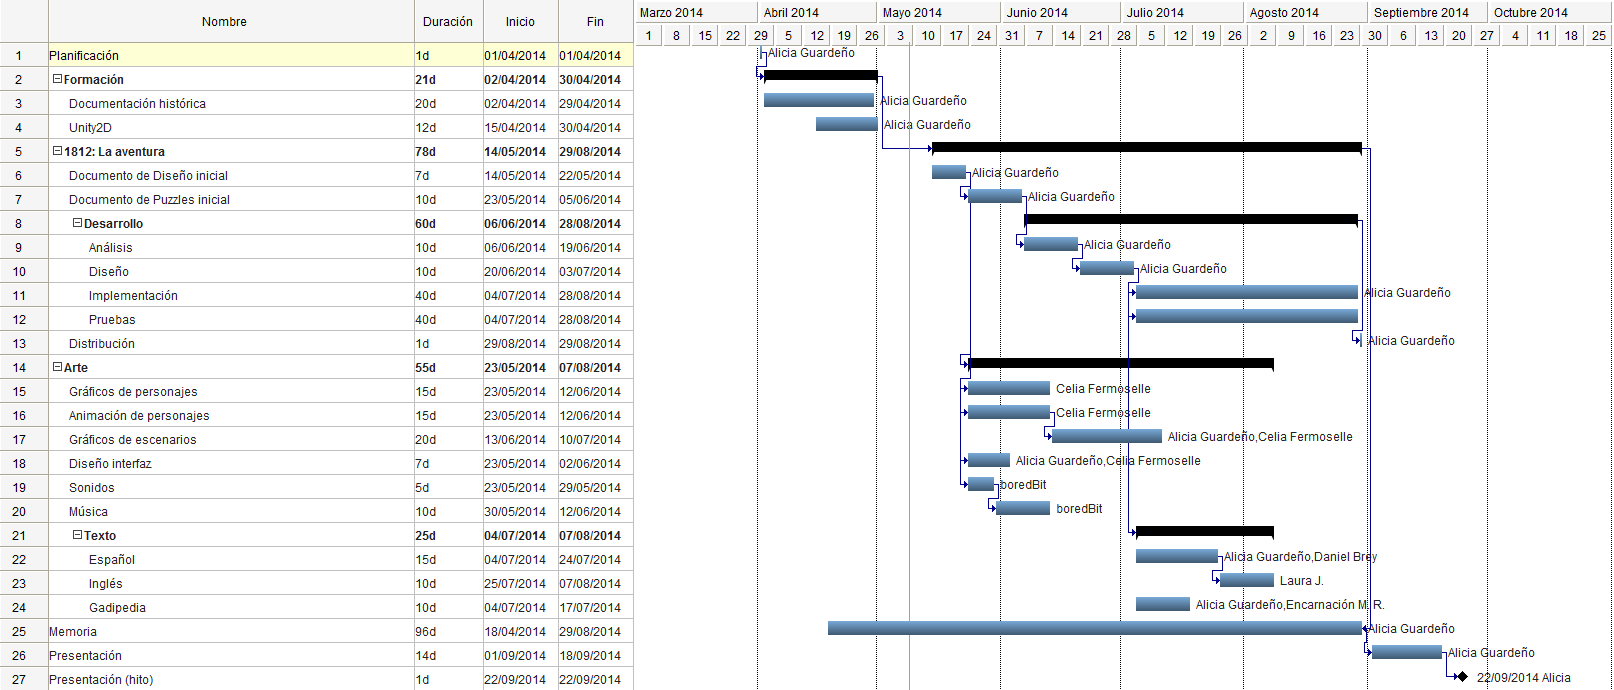
\includegraphics[scale=0.4]{planificacionv2-1.png}
    \makebox[\textwidth]{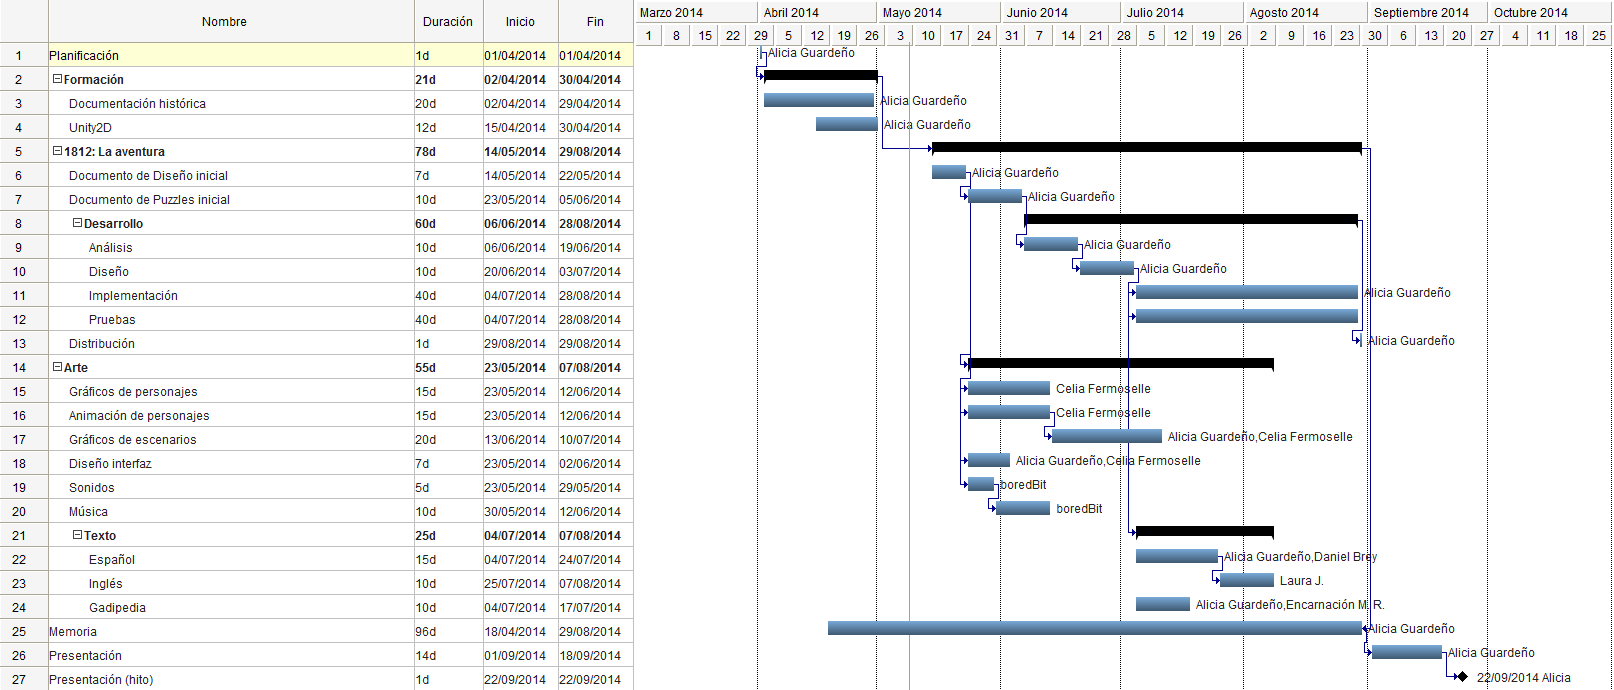
\includegraphics[width=0.9\paperwidth]{planificacionv2-1.png}}
  \end{center}
  \caption{Planificación del proyecto desde abril de 2014 hasta septiembre de 2014}
    \label{fig:gantt}
\end{figure}

\section{Etapas de desarrollo del proyecto}

\begin{enumerate}
\item\negrita{Planificación} \hfill \\
Dada la envergadura del proyecto, era necesaria una etapa de planificación en la que se ha estudiado de forma cuidadosa el alcance del mismo y las posibles dificultades a encontrar durante el desarrollo.

\item\negrita{Formación} \hfill \\
Al comienzo del proyecto desconocía por completo el uso de \programa{Unity3D} y su API, el lenguaje C\#. Además de carecer de conocimientos históricos profundos sobre el Cádiz en la época de 1812. Fue necesaria, por tanto, una larga etapa de formación personal utilizando varios recursos bibliográficos, tanto históricos como para desarrollo de videojuegos, y pequeñas pruebas prácticas en \programa{Unity3D}.

\item\negrita{1812: La aventura} \hfill \\
Tras el periodo de aprendizaje, se comenzó con el videojuego \nombrejuego{}. El primer paso fue crear una cuenta en la forja de \programa{GitHub}. Dicha forja proporciona un repositorio \emph{Git} y herramientas web que ayudan en la gestión de un proyecto: gestor de tareas, subida de ficheros, publicación de noticias, wiki, foros, etc.

\begin{enumerate}
\item \emph{Documento de diseño} \hfill \\
En el documento de diseño de un videojuego se detallan elementos como la historia, género, personajes, mecánicas de juego, objetos o escenarios entre otros muchos. En definitiva, es el documento que define de forma más o menos concisa cómo será el videojuego. Se trata de un escrito muy importante ya que ayuda a que todo el equipo albergue la misma idea sobre el videojuego y pueda trabajar de forma más compenetrada.

\item \emph{Documento de puzzles} \hfill \\
En el documento de puzzles de un videojuego, más propiamente de una aventura gráfica, en la que se detallas los puzzles, la jerarquía de resolución de puzzles, escenarios y objetos involucrados en su resolución. Se trata de un escrito muy importante ya que determina el flujo del desarrollo de una aventura gráfica, y lo entretenido que pueda llegar a ser para un usuario.

\item \emph{Análisis} \hfill \\
La fase de análisis dió comienzo después de la redacción y revisión de los documentos de diseño y puzzles. Se procedió con la toma de requisitos a partir de dicho documento, se confeccionaron los casos de uso, se elaboró el modelo conceptual de datos y se detalló el modelo de comportamiento.

\item \emph{Diseño} \hfill \\
Durante la fase de diseño, que siguió de forma inmediata al análisis, se elaboraron los diagramas de clases.

\item \emph{Implementación} \hfill \\
La fase de implementación de \nombrejuego{} fue, con diferencia, la más extendida de todo el desarrollo. Quizás viniese motivada por la inexperiencia y los varios sistemas, entre ellos una pequeña base de datos,  que se tuvieron que implementar desde la base.

\item \emph{Pruebas} \hfill \\
Durante la implementación se fueron realizando pruebas de módulos individuales pero fue tras finalizar dicha fase cuando tuvieron lugar las pruebas de integración. No sólo se trabajó para que el código fuese correcto, sino que \nombrejuego{} fue probado de forma extensiva por colaboradores distintos al desarrollador principal con el claro objetivo de pulir ciertos detalles relacionados como el balanceo de la dificultad de los puzzles (que no sean ni fáciles ni difíciles), el correcto control del personaje entre otras cosas.

%\item \emph{Mantenimiento} \hfill \\
%

\item \emph{Distribución} \hfill \\
Se crearon y publicaron paquetes descargables para los sistemas GNU/Linux, MacOSX y Windows. Por suerte \programa{Unity3D} es un editor que cuenta con un compilador multiplataforma, con lo que solo tomó un día en crear todos los paquetes.  
%

\item \emph{Arte} \hfill \\
El proceso de creación la mayor parte del arte necesario para \nombrejuego{} comenzó nada más acabar la redacción del documento de diseño, exceptuándo algunas partes del guión que eran dependientes de la finalización del documento de puzzles. Desde el momento que se tenía completado el documento de diseño, se conocía el estilo visual del juego, los escenarios, personajes y música que aparecerían. Por su complejidad, el trabajo se extendió prácticamente durante todo el desarrollo. Al ser la única tarea en la que participaron colaboradores, fueron necesarias labores de supervisión y coordinación: estilo, formato de entrega, corrección de fallos, etc.

\begin{enumerate}
\item \emph{Gráficos de personajes} \hfill \\
Los gráficos los realizó Celia Fermoselle, realizados con la técnica de \cursiva{pixel art} dado que era como mejor y más rápido trabajaba. La coordinación en este punto fue crítica pues había que llegar a una estética que gustase al público y que a su vez fuera sencillo de realizar.

\item \emph{Animación de personajes} \hfill \\
Una vez finalizados los gráficos de los personajes, Celia tuvo que hacer su animación por cuadros. Esta técnica se basa en modificar los gráficos originales en sucesivos cuadros, que al repetirse rápidamente dan ilusión de movimiento. Teniendo el estilo ya definido de los primeros gráficos, la supervisión y coordinación no fue tan cargante.

\item \emph{Gráficos de escenarios} \hfill \\
Aquí el trabajo fue realizado por un grupo: Celia se encargaba de realizar los escenarios en \cursiva{pixel art}, mientras tanto, yo le pasaba fotos de escenarios reales en los que basarse y los bocetos de los escenarios ficticios a partir de las fotos. Para poder realizar las fotos, fue necesaria la ayuda de [...], perteneciente a la Asociación de Recreación Histórica del Cádiz de 1812, el cual nos facilitó el acceso a trajes, armas, sitios de relevancia de la época, etc.

\item \emph{Diseño de la interfaz} \hfill \\
A partir del documento de diseño, la interfaz fue realizada rápidamente por Celia Fermoselle.

\item \emph{Efectos de sonido} \hfill \\
Una vez detallados los sonidos requeridos en el documento de diseño, estos fueron realizados por el equipo de músicos boredBit.

\item \emph{BSO} \hfill \\
Ya acabados los sonidos principales del juego, boredBit se dispuso a realizar la música del juego. La coordinación fue necesaria, para en el mismo caso que los gráficos, se definiera un estilo de música que fue incluido el documento de diseño.


\item \emph{Texto} \hfill \\
Siendo \nombrejuego{} una aventura gráfica, la calidad de los diálogos y descripciones es necesaria para ser disfrutado por el público y ayudar a la resolución de puzzles. Daniel Brey se prestó a colaborar conmigo para la realización de estos fijándonos en el documento de diseño y de puzzles, también Encarnación M. R. que asesoró que no hubiera incongruencias en los contenidos relacionados con el Cádiz de 1812.

\begin{enumerate}
\item \emph{Español} \hfill \\
Tal y como se ha dicho en el apartado anterior, Daniel Brey realizó el guión del videojuego en español sirviéndose del documento de diseño y puzzles, además de contar con mi ayuda y la de Encarnación M. R. en temas históricos.

\item \emph{Inglés} \hfill \\
Finalizado los textos en español, Laura J. Torres procedió a transcribirlos al inglés. Durante la transcripción, fue necesaria la coordinación para indicarle el formato que tenía que seguir el texto. Posteriormente ayudó en la realización de un documento que dictase los pasos a seguir para modificar los textos o traducirlos a otros idiomas más adelante.

\item \emph{Gadipedia} \hfill \\
La extraña palabra Gadipedia viene a ser una pequeña enciclopedia de los hechos más importantes de la época del Cádiz de 1812, además de incluir algunas anécdotas que nos ayudan a vislumbrar la vida cotidiana de entonces como los uniformes, el comercio, etc. Todo ello accesible desde dentro del juego para ayudar a la resolución de los puzzles. Ahora bien, si la parte de la implementación corrió a cuenta mía, la de la generación y supervisión de los textos fue gracias a Encarnación M. R.

\end{enumerate}

\end{enumerate}

\end{enumerate}

\item\negrita{Memoria} \hfill \\
Antes, durante y después del desarrollo de \nombrejuego{} se procedió a la redacción del presente documento que incluye apéndices adicionales como el manual de usuario del videojuego.

\item\negrita{Presentación} \hfill \\
Como última tarea en la organización temporal figura la elaboración de la exposición de cara a la presentación del \negrita{Proyecto fin de Carrera}. Se llevó a cabo tratando de plasmar el trabajo realizado y los objetivos conseguidos con el desarrollo de este proyecto.

\item\negrita{Comunidad} \hfill \\
Una de las partes fundamentales de este proyecto es su objetivo de servir a la comunidad. Hasta el momento había una escasa documentación sobre cómo diseñar un videojuego en español, más concretamente al diseño de las aventuras gráficas. A lo largo de todo el desarrollo ha estado presente la atención e interacción con la comunidad a través de diversos medios como redes sociales, foros de desarrolladores de videojuegos y el blog.

\item\negrita{Presentación (hito)} \hfill \\
Finalmente, el día [...] se entrega toda la documentación del proyecto y se preparó la presentación final que tendría lugar, aproximadamente, [...] después.

\end{enumerate}


%\chapter{Desarrollo de 1812: La aventura}
%\label{chap:desarrollo}
%
\section{Metodología}
\nombrejuego será un sistema software complejo y para su desarrollo se ha decidido emplear la metodología . Así mismo, se ha escogido \emph{UML} como la notación para modelar nuestro sistema.

Mediante la metodología [] podemos realizar un desarrollo orientado a objetos de forma iterativa. Las ventajas que nos proporciona el paradigma de la orientación a objetos consisten en una mayor reusabilidad (uno de los objetivos principales del juego), escalabilidad, legilibilidad y sencillez de mantenimiento.

\section{Análisis}
\subsection{Especificación de requisitos del sistema}


%\chapter{Conclusiones}
%\label{chap:conclusiones}
%\input{conclusiones.tex}

%\addcontentsline{toc}{chapter}{Software usado}
\chapter*{Software utilizado}
\label{chap:software}
% -*-programas.tex-*-
% Este fichero es parte de la plantilla LaTeX para
% la realización de Proyectos Final de Carrera, protejido
% bajo los términos de la licencia GFDL.
% Para más información, la licencia completa viene incluida en el
% fichero fdl-1.3.tex

% Copyright (C) 2009 Pablo Recio Quijano 


%Es usual en un PFC referenciar que software has usado para la
%realización del mismo. Aprovecharé este apartado para que conozcas
%alguna herramienta que puede serte de ayuda para realizar tus
%documentos en \LaTeX{}

%\section*{Emacs + Auc\TeX}

%Emacs es uno de los programas de edición más usados por
%desarrolladores de software, ya que es bastante versatil admitiendo
%gran cantidad de ``plugins'' o extensiones que permiten ampliar aun
%más sus funcionalidades.\\

%Uno de estos plugins es Auc\TeX \cite{pdf:auctex}, el cual incluye
%rutas para ciertos comandos, resaltado de sintaxis, previsualización
%del documento, menú matemático en el cual podemos acceder e insertar
%la gran mayoria de los símbolos matemáticos, para no tener que
%memorizarlos. Podemos ver un ejemplo de Emacs + Auc\TeX en la figura
%\ref{auctex}

%\figura{Auctex.png}{scale=0.6}{Emacs + Auc\TeX}{auctex}{h}

%Por ejemplo, para cerrar un entorno $\backslash$\texttt{begin()}, con su
%respectivo $\backslash$\texttt{end()}, utilizaremos el atajo
%\comando{C-c M-]}, para añadir un $\backslash$\texttt{item}, tenemos
%el atajo \comando{C-c C-j}, y así unos cuantos, que una vez que nos
%habituamos a ellos, son bastante cómodos.\\

%Además, es bastante configurable, con indentado automático, corrector
%ortográfico y demás. El fichero adjunto a este documento,
%\emph{conf\_emacs} incluye una configuración con varias de estas
%opciones.

%\section*{Doxygen}

%Realmente, \programa{Doxygen} \cite{website:doxygen} no es una herramienta
%que vayamos a utilizar para realizar documentos \LaTeX{}
%directamente. Sin embargo, para la documentación de código si es
%bastante útil.\\

%Esta herramienta realiza una documentación automática de código
%fuente. Es decir, para nuestro PFC, podemos utilizar para generar la
%documentación de las APIs de nuestras librerías y demás. Puede generar
%esta documentación en varios formatos, y entre ellos, \LaTeX, de forma
%que podemos utilizar ese código generado en nuestra memoria de forma
%automática.

%\section*{GNU Make}

%\programa{GNU Make} es el programa de recompilación y de control de
%dependencias por excelencia. Se puede utilizar para compilar proyectos
%software en diversos códigos, o como en el caso de este documento,
%para compilar documentos \LaTeX{} con diversas opciones.\\

%Para más información \cite{pdf:make}

%\section*{Dia}

%\programa{Dia} es un editor de gráficos vectoriales el cual incluye
%distintas plantillas para distintos tipos de gráficos, como pueden ser
%UML, ERe, diagramas de flujo, esquemas Cisco de red y un larguísimo
%etcétera. Podemos ver el interfaz en la figura \ref{dia}

%\figura{dia.png}{scale=0.6}{Interfaz de Dia}{dia}{h}

%Estos diagramas podemos exportarlos a diversos formatos de imagen
%(\texttt{.png}, \texttt{.eps}, ...) o a formato \texttt{.tex}, como
%vimos anteriormente.

% % % % % % % % % % % % % % % % % % % % % % % % % % % % % % % % % % % % % % % % %
En esta sección hablaremos de las herramientas utilizadas durante el desarrollo de \nombrejuego. Para cada herramienta ofreceremos una pequeña descripción de sus funcionalidades y adjuntaremos las razones por las cuales han sido elegidos para el desarrollo frente a otros de similares características.


\section*{Unity}

\section*{Doxygen}
\programa{Doxygen} \cita{doxygen} es una herramienta de documentación automática de código. Mediante la inclusión de comentarios especiales dentro de los ficheros de nuestro proyecto, es capaz de generar documentación con una apariencia atractiva tanto en formato HTML, como en \LaTeX o muchos otros. Es compatible con los lenguajes C, C++, C\#, Frortran, Java, Objective-C, PHP, Python, IDL y algunos más.

Con \programa{Doxygen} se produce una documentación legible por usuarios (con los conocimientos necesarios) u otros miembros del equipo. Es posible incluir diagramas de colaboración y herencia gracias a su uso de GraphViz. Ha sido elegida como herramienta de documentación de código por su sencillez de uso, limpieza y por su amplia aceptación.

\section*{LaTeX + TeXstudio}
\LaTeX \cita{latex-project} es un lenguaje de marcado y un sistema de creación de documentos especialmente orientado al mundo científico y técnico. El lenguaje \programa{Tex} fue concebido por Donald Knuth durante los 80 y en 1984 Leslie Lamport creó \LaTeX como un framework para trabajar con cartas, libros y otro tipo de textos.

Los resultados que produce \LaTeX son coherentes, ordenados y muy limpios. Si bien aprender su uso puede ser complejo, los resultados son de una enorme calidad si los comparamos con los documentos que producen los editores convenciones como \programa{Microsoft Word} o \programa{LibreOffice Writer}. Por esta calidad y posibilidad de automatizar formatos ha sido elegido \LaTeX para la redacción de la documentación del proyecto.

En un principio se eligió ShareLaTeX \cita{sharelatex} como el editor de la documentación el \LaTeX de \nombrejuego. Pues es un editor online con herramientas colaborativas y que permite compilar en cualquier equipo al guardarse como si fuera una copia de seguridad. Pero ante el nulo uso colaborativo a la hora de la verdad, los diversos problemas de sincronizar los cambios y de compilar cuando la página se satura de usuarios, finalmente hicieron que optara por otro editor. 

En este caso el ganador resultó ser TeXstudio \cita{texstudio}, un editor multiplataformas libre, cuya interfaz es cómoda a la hora de visualizar la estructura de los ficheros que componen la documentación, además de incluir corrector ortográfico y sintáctico, autocompletado, herramientas avanzadas de resaltado y editado de texto, un visor de PDF integrado y otras muchas más características.

\section*{Microsoft Visual Studio Express 2013 + UnityVSExpress}
\programa{Microsoft Visual Studio Express 2013} \cita{visual-studio-express} es un programa de desarrollo en entorno de desarrollo integrado (IDE en inglés) para sistemas operativos Windows desarrollado y distribuido por Microsoft Corporation. Soporta varios lenguajes tales como Visual C++, Visual Basic .NET, y a destacar el usado en \nombrejuego que es C\# aunque actualmente se han desarrollado las extensiones necesarias para muchos otros. Es de carácter gratuito y es proporcionado por la compañía Microsoft Corporation.

Los motivos de su elección son, que a pesar de que \programa{Unity} incluya su propio IDE llamado Monodevelop \cita{monodevelop}, que si bien para trabajos sencillos cumple con las expectativas, a la hora de embarcarnos en un proyecto con mayor carga de código tiene problemas a la hora de navegar entre las extensas líneas de código, abrir ficheros del proyecto manualmente, resultando poco eficiente. Así que teniendo en cuenta que el SO con el que se va a desarrollar es Windows dado que \programa{Unity} aún no ha lanzado su editor para plataformas GNU/Linux, se optó por \programa{Microsoft Visual Studio Express 2013}, uno de los IDE más utilizados en Windows, y por ende, en muchas empresas. Ha sido utilizado para el proyecto por su completa herramienta de depuración, corrector ortográfico, autocompletado, entre otras cualidades que han ayudado a mejorar la productividad.

Además en este caso, se hace uso del plugin \programa{UnityVSExpress} \cita{unityvsexpress} que permite la integración de \programa{Microsoft Visual Studio Express 2013} en los proyectos de \programa{Unity} desarrollados en C\#. Facilitando más aún el trabajo a la hora de redactar el código para \nombrejuego.

\section*{Git + GitHub + Git Shell}
\programa{Git} \cita{git} es un sistema de control de versiones libre enfocado en flujos de trabajo no lineales, integridad de datos y rapidez. Inicialmente fue diseñado y desarrollado por Linus Torvals para el kernel de Linux en 2005, y desde entonces se ha convertido en el sistema de control de versiones más usado para el desarrollo de software. \programa{Git} nos permite contar con una copia de seguridad del código de \nombrejuego en todo momento. Gracias a esta herramienta podemos guardar un historial de todas las versiones de los ficheros, así como deshacer cambios en caso de que fuera necesario. También permite crear ramas con distintas versiones del proyecto y luego fusionarlas en otra. Con \programa{Git} conseguimos acceso al código del proyecto desde cualquier equipo. Además, pone a disposición de cualquier interesado el código fuente de forma sencilla.

Existen otros sistemas de control de versiones como \programa{Subversion} o \programa{Mercurial}. Se ha elegido \programa{Git} para aprender a desarrollar en este sistema de control de versiones, al ser el más extendido y requerido a la hora de trabajar en equipos con varios programadores en un proyecto de software. 

Además de \programa{Git}, se ha elegido la forja \programa{GitHub} \cita{github} que usa dicho sistema de control de versiones. Los motivos son que al ser la forja más popular y reconocida a fecha de hoy, e incluir elementos sociales, permite una mayor difusión del proyecto. \programa{GitHub} también proporciona su propia herramienta para Windows, llamada GitHub Windows \cita{github-windows}, con la que gestionar el control de versiones de manera sencilla y visual para los más novatos. Para los más experimentados y familiarizados de UNIX, incluye la herramienta Git Shell que es una terminal para Windows que permite la utilización de los comandos bash de \programa{Git}. 

Existe otra herramienta llamada también Git Shell \cita{git-for-windows}, siendo esta la oficial usada en el proyecto \programa{Git}, pero por comodidad y sencillez se ha optado por la terminal Git Shell de \programa{GitHub}.

\section*{GraphicsGale FreeEdition}
\programa{GraphicsGale} \cita{graphicsgale} es un editor de gráficos orientados al pixel-art para Windows. Permite la utilización de capas, un sistema de animación (con capas de cebolla para facilitar la creación de animaciones), otras muchas características específicas para el uso del pixel-art tales como el control de la paleta de colores.

Ha sido utilizado para la creación y edición de los gráficos de \nombrejuego con estética pixel-art. Siendo elegido por ser un editor muy completo y potente para este tipo de gráficos.

\section*{GIMP}
\programa{GIMP} \cita{gimp} es el editor de imágenes libre del proyecto GNU, de hecho su nombre es un acrónimo de \emph{GNU image Manipulation Program}. Es multiplataforma y está disponible para Windows, GNU/Linux y Mac OS X. No es comparable a soluciones provativas como \programa{Adobe Photoshop} pero es capaz de realizar operaciones bastante avanzadas de forma sencilla.

Ha sido utilizado en \nombrejuego para crear las transparencias necesarias en las hojas de sprites realizados con \programa{GraphicsGale}. Hemos elegido esta herramienta por contar con una licencia libre, ser lo suficientemente potente para nuestras necesidades y estar disponible en varias plataformas.

\section*{Cacoo}

\section*{Gantter}

%\addcontentsline{toc}{chapter}{Instalación de \LaTeX}
%\chapter*{Instalación de \LaTeX}
%% -*-instalacion.tex-*-
% Este fichero es parte de la plantilla LaTeX para
% la realización de Proyectos Final de Carrera, protejido
% bajo los términos de la licencia GFDL.
% Para más información, la licencia completa viene incluida en el
% fichero fdl-1.3.tex

% Copyright (C) 2009 Pablo Recio Quijano 

Veamos que tenemos que hacer para instalar \LaTeX{} con todas sus
capacidades en un sistema basado en Debian, como Ubuntu.
Primero hay que tener en cuenta que \LaTeX{} es relativamente pesado
con respecto a otros compiladores. \\

Nosotros vamos a utilizar la distribución de \LaTeX{} incluida en los
repositorios de Ubuntu llamada \programa{texlive}. Si la buscas en
tu gestor de paquetes, encontrarás infinidad de paquetes aparte
del principal. Existen otras distribuciones como Te\TeX\\

Si instalas solo los básicos, es decir instalas \programa{texlive} y
los programas necesarios para él, no podrás compilar este documento,
ya que faltarian paquetes tales como \programa{supertabular} y
varios. Por eso, si no tienes problema de espacio en el disco duro te
recomiendo que instales el paquete \programa{texlive-full}, que
instala \negrita{todos} los paquetes de \programa{texlive}, incluyendo
documentación en todos los idiomas disponibles. Si buscas no tener
problemas de dependencias, este es tu método.\\

\begin{lstlisting}[style=consola]
  sudo apt-get install texlive-full
\end{lstlisting}

En caso de querer ser un poco más concreto, en principio puedes
trabajar con la más básica (\programa{texlive} y sus dependencias) y
en función de los paquetes que te vayan faltando, los instalas.

% TO-DO: paquetes concretos e instalación en otros sistemas

%-------------------------------------------------
\setlength{\parskip}{0cm} %Lo pongo aqui para evitar el salto de línea en los índices
%-------------------------------------------------

\backmatter % Apéndices, bibliografia ...


\clearpage
\addcontentsline{toc}{chapter}{Bibliografía y referencias}
%\cite{website:example}
\bibliography{bibliografia}{}
\bibliographystyle{plain}
%\printbibliography

% This is set up to run with pdflatex.
%---------The file header---------------------------------------------
%---------------------------------------------------------------------
\chapter*{\rlap{GNU Free Documentation License}}
\phantomsection  % so hyperref creates bookmarks
\addcontentsline{toc}{chapter}{GNU Free Documentation License}
%\label{label_fdl}

 \begin{center}

       Version 1.3, 3 November 2008


 Copyright \copyright{} 2000, 2001, 2002, 2007, 2008  Free Software Foundation, Inc.
 
 \bigskip
 
     <http://fsf.org/>
  
 \bigskip
 
 Everyone is permitted to copy and distribute verbatim copies
 of this license document, but changing it is not allowed.
\end{center}


\begin{center}
{\bf\large Preamble}
\end{center}

The purpose of this License is to make a manual, textbook, or other
functional and useful document ``free'' in the sense of freedom: to
assure everyone the effective freedom to copy and redistribute it,
with or without modifying it, either commercially or noncommercially.
Secondarily, this License preserves for the author and publisher a way
to get credit for their work, while not being considered responsible
for modifications made by others.

This License is a kind of ``copyleft'', which means that derivative
works of the document must themselves be free in the same sense.  It
complements the GNU General Public License, which is a copyleft
license designed for free software.

We have designed this License in order to use it for manuals for free
software, because free software needs free documentation: a free
program should come with manuals providing the same freedoms that the
software does.  But this License is not limited to software manuals;
it can be used for any textual work, regardless of subject matter or
whether it is published as a printed book.  We recommend this License
principally for works whose purpose is instruction or reference.


\begin{center}
{\Large\bf 1. APPLICABILITY AND DEFINITIONS\par}
\phantomsection
\addcontentsline{toc}{section}{1. APPLICABILITY AND DEFINITIONS}
\end{center}

This License applies to any manual or other work, in any medium, that
contains a notice placed by the copyright holder saying it can be
distributed under the terms of this License.  Such a notice grants a
world-wide, royalty-free license, unlimited in duration, to use that
work under the conditions stated herein.  The ``\textbf{Document}'', below,
refers to any such manual or work.  Any member of the public is a
licensee, and is addressed as ``\textbf{you}''.  You accept the license if you
copy, modify or distribute the work in a way requiring permission
under copyright law.

A ``\textbf{Modified Version}'' of the Document means any work containing the
Document or a portion of it, either copied verbatim, or with
modifications and/or translated into another language.

A ``\textbf{Secondary Section}'' is a named appendix or a front-matter section of
the Document that deals exclusively with the relationship of the
publishers or authors of the Document to the Document's overall subject
(or to related matters) and contains nothing that could fall directly
within that overall subject.  (Thus, if the Document is in part a
textbook of mathematics, a Secondary Section may not explain any
mathematics.)  The relationship could be a matter of historical
connection with the subject or with related matters, or of legal,
commercial, philosophical, ethical or political position regarding
them.

The ``\textbf{Invariant Sections}'' are certain Secondary Sections whose titles
are designated, as being those of Invariant Sections, in the notice
that says that the Document is released under this License.  If a
section does not fit the above definition of Secondary then it is not
allowed to be designated as Invariant.  The Document may contain zero
Invariant Sections.  If the Document does not identify any Invariant
Sections then there are none.

The ``\textbf{Cover Texts}'' are certain short passages of text that are listed,
as Front-Cover Texts or Back-Cover Texts, in the notice that says that
the Document is released under this License.  A Front-Cover Text may
be at most 5 words, and a Back-Cover Text may be at most 25 words.

A ``\textbf{Transparent}'' copy of the Document means a machine-readable copy,
represented in a format whose specification is available to the
general public, that is suitable for revising the document
straightforwardly with generic text editors or (for images composed of
pixels) generic paint programs or (for drawings) some widely available
drawing editor, and that is suitable for input to text formatters or
for automatic translation to a variety of formats suitable for input
to text formatters.  A copy made in an otherwise Transparent file
format whose markup, or absence of markup, has been arranged to thwart
or discourage subsequent modification by readers is not Transparent.
An image format is not Transparent if used for any substantial amount
of text.  A copy that is not ``Transparent'' is called ``\textbf{Opaque}''.

Examples of suitable formats for Transparent copies include plain
ASCII without markup, Texinfo input format, LaTeX input format, SGML
or XML using a publicly available DTD, and standard-conforming simple
HTML, PostScript or PDF designed for human modification.  Examples of
transparent image formats include PNG, XCF and JPG.  Opaque formats
include proprietary formats that can be read and edited only by
proprietary word processors, SGML or XML for which the DTD and/or
processing tools are not generally available, and the
machine-generated HTML, PostScript or PDF produced by some word
processors for output purposes only.

The ``\textbf{Title Page}'' means, for a printed book, the title page itself,
plus such following pages as are needed to hold, legibly, the material
this License requires to appear in the title page.  For works in
formats which do not have any title page as such, ``Title Page'' means
the text near the most prominent appearance of the work's title,
preceding the beginning of the body of the text.

The ``\textbf{publisher}'' means any person or entity that distributes
copies of the Document to the public.

A section ``\textbf{Entitled XYZ}'' means a named subunit of the Document whose
title either is precisely XYZ or contains XYZ in parentheses following
text that translates XYZ in another language.  (Here XYZ stands for a
specific section name mentioned below, such as ``\textbf{Acknowledgements}'',
``\textbf{Dedications}'', ``\textbf{Endorsements}'', or ``\textbf{History}''.)  
To ``\textbf{Preserve the Title}''
of such a section when you modify the Document means that it remains a
section ``Entitled XYZ'' according to this definition.

The Document may include Warranty Disclaimers next to the notice which
states that this License applies to the Document.  These Warranty
Disclaimers are considered to be included by reference in this
License, but only as regards disclaiming warranties: any other
implication that these Warranty Disclaimers may have is void and has
no effect on the meaning of this License.


\begin{center}
{\Large\bf 2. VERBATIM COPYING\par}
\phantomsection
\addcontentsline{toc}{section}{2. VERBATIM COPYING}
\end{center}

You may copy and distribute the Document in any medium, either
commercially or noncommercially, provided that this License, the
copyright notices, and the license notice saying this License applies
to the Document are reproduced in all copies, and that you add no other
conditions whatsoever to those of this License.  You may not use
technical measures to obstruct or control the reading or further
copying of the copies you make or distribute.  However, you may accept
compensation in exchange for copies.  If you distribute a large enough
number of copies you must also follow the conditions in section~3.

You may also lend copies, under the same conditions stated above, and
you may publicly display copies.


\begin{center}
{\Large\bf 3. COPYING IN QUANTITY\par}
\phantomsection
\addcontentsline{toc}{section}{3. COPYING IN QUANTITY}
\end{center}


If you publish printed copies (or copies in media that commonly have
printed covers) of the Document, numbering more than 100, and the
Document's license notice requires Cover Texts, you must enclose the
copies in covers that carry, clearly and legibly, all these Cover
Texts: Front-Cover Texts on the front cover, and Back-Cover Texts on
the back cover.  Both covers must also clearly and legibly identify
you as the publisher of these copies.  The front cover must present
the full title with all words of the title equally prominent and
visible.  You may add other material on the covers in addition.
Copying with changes limited to the covers, as long as they preserve
the title of the Document and satisfy these conditions, can be treated
as verbatim copying in other respects.

If the required texts for either cover are too voluminous to fit
legibly, you should put the first ones listed (as many as fit
reasonably) on the actual cover, and continue the rest onto adjacent
pages.

If you publish or distribute Opaque copies of the Document numbering
more than 100, you must either include a machine-readable Transparent
copy along with each Opaque copy, or state in or with each Opaque copy
a computer-network location from which the general network-using
public has access to download using public-standard network protocols
a complete Transparent copy of the Document, free of added material.
If you use the latter option, you must take reasonably prudent steps,
when you begin distribution of Opaque copies in quantity, to ensure
that this Transparent copy will remain thus accessible at the stated
location until at least one year after the last time you distribute an
Opaque copy (directly or through your agents or retailers) of that
edition to the public.

It is requested, but not required, that you contact the authors of the
Document well before redistributing any large number of copies, to give
them a chance to provide you with an updated version of the Document.


\begin{center}
{\Large\bf 4. MODIFICATIONS\par}
\phantomsection
\addcontentsline{toc}{section}{4. MODIFICATIONS}
\end{center}

You may copy and distribute a Modified Version of the Document under
the conditions of sections 2 and 3 above, provided that you release
the Modified Version under precisely this License, with the Modified
Version filling the role of the Document, thus licensing distribution
and modification of the Modified Version to whoever possesses a copy
of it.  In addition, you must do these things in the Modified Version:

\begin{itemize}
\item[A.] 
   Use in the Title Page (and on the covers, if any) a title distinct
   from that of the Document, and from those of previous versions
   (which should, if there were any, be listed in the History section
   of the Document).  You may use the same title as a previous version
   if the original publisher of that version gives permission.
   
\item[B.]
   List on the Title Page, as authors, one or more persons or entities
   responsible for authorship of the modifications in the Modified
   Version, together with at least five of the principal authors of the
   Document (all of its principal authors, if it has fewer than five),
   unless they release you from this requirement.
   
\item[C.]
   State on the Title page the name of the publisher of the
   Modified Version, as the publisher.
   
\item[D.]
   Preserve all the copyright notices of the Document.
   
\item[E.]
   Add an appropriate copyright notice for your modifications
   adjacent to the other copyright notices.
   
\item[F.]
   Include, immediately after the copyright notices, a license notice
   giving the public permission to use the Modified Version under the
   terms of this License, in the form shown in the Addendum below.
   
\item[G.]
   Preserve in that license notice the full lists of Invariant Sections
   and required Cover Texts given in the Document's license notice.
   
\item[H.]
   Include an unaltered copy of this License.
   
\item[I.]
   Preserve the section Entitled ``History'', Preserve its Title, and add
   to it an item stating at least the title, year, new authors, and
   publisher of the Modified Version as given on the Title Page.  If
   there is no section Entitled ``History'' in the Document, create one
   stating the title, year, authors, and publisher of the Document as
   given on its Title Page, then add an item describing the Modified
   Version as stated in the previous sentence.
   
\item[J.]
   Preserve the network location, if any, given in the Document for
   public access to a Transparent copy of the Document, and likewise
   the network locations given in the Document for previous versions
   it was based on.  These may be placed in the ``History'' section.
   You may omit a network location for a work that was published at
   least four years before the Document itself, or if the original
   publisher of the version it refers to gives permission.
   
\item[K.]
   For any section Entitled ``Acknowledgements'' or ``Dedications'',
   Preserve the Title of the section, and preserve in the section all
   the substance and tone of each of the contributor acknowledgements
   and/or dedications given therein.
   
\item[L.]
   Preserve all the Invariant Sections of the Document,
   unaltered in their text and in their titles.  Section numbers
   or the equivalent are not considered part of the section titles.
   
\item[M.]
   Delete any section Entitled ``Endorsements''.  Such a section
   may not be included in the Modified Version.
   
\item[N.]
   Do not retitle any existing section to be Entitled ``Endorsements''
   or to conflict in title with any Invariant Section.
   
\item[O.]
   Preserve any Warranty Disclaimers.
\end{itemize}

If the Modified Version includes new front-matter sections or
appendices that qualify as Secondary Sections and contain no material
copied from the Document, you may at your option designate some or all
of these sections as invariant.  To do this, add their titles to the
list of Invariant Sections in the Modified Version's license notice.
These titles must be distinct from any other section titles.

You may add a section Entitled ``Endorsements'', provided it contains
nothing but endorsements of your Modified Version by various
parties---for example, statements of peer review or that the text has
been approved by an organization as the authoritative definition of a
standard.

You may add a passage of up to five words as a Front-Cover Text, and a
passage of up to 25 words as a Back-Cover Text, to the end of the list
of Cover Texts in the Modified Version.  Only one passage of
Front-Cover Text and one of Back-Cover Text may be added by (or
through arrangements made by) any one entity.  If the Document already
includes a cover text for the same cover, previously added by you or
by arrangement made by the same entity you are acting on behalf of,
you may not add another; but you may replace the old one, on explicit
permission from the previous publisher that added the old one.

The author(s) and publisher(s) of the Document do not by this License
give permission to use their names for publicity for or to assert or
imply endorsement of any Modified Version.


\begin{center}
{\Large\bf 5. COMBINING DOCUMENTS\par}
\phantomsection
\addcontentsline{toc}{section}{5. COMBINING DOCUMENTS}
\end{center}


You may combine the Document with other documents released under this
License, under the terms defined in section~4 above for modified
versions, provided that you include in the combination all of the
Invariant Sections of all of the original documents, unmodified, and
list them all as Invariant Sections of your combined work in its
license notice, and that you preserve all their Warranty Disclaimers.

The combined work need only contain one copy of this License, and
multiple identical Invariant Sections may be replaced with a single
copy.  If there are multiple Invariant Sections with the same name but
different contents, make the title of each such section unique by
adding at the end of it, in parentheses, the name of the original
author or publisher of that section if known, or else a unique number.
Make the same adjustment to the section titles in the list of
Invariant Sections in the license notice of the combined work.

In the combination, you must combine any sections Entitled ``History''
in the various original documents, forming one section Entitled
``History''; likewise combine any sections Entitled ``Acknowledgements'',
and any sections Entitled ``Dedications''.  You must delete all sections
Entitled ``Endorsements''.

\begin{center}
{\Large\bf 6. COLLECTIONS OF DOCUMENTS\par}
\phantomsection
\addcontentsline{toc}{section}{6. COLLECTIONS OF DOCUMENTS}
\end{center}

You may make a collection consisting of the Document and other documents
released under this License, and replace the individual copies of this
License in the various documents with a single copy that is included in
the collection, provided that you follow the rules of this License for
verbatim copying of each of the documents in all other respects.

You may extract a single document from such a collection, and distribute
it individually under this License, provided you insert a copy of this
License into the extracted document, and follow this License in all
other respects regarding verbatim copying of that document.


\begin{center}
{\Large\bf 7. AGGREGATION WITH INDEPENDENT WORKS\par}
\phantomsection
\addcontentsline{toc}{section}{7. AGGREGATION WITH INDEPENDENT WORKS}
\end{center}


A compilation of the Document or its derivatives with other separate
and independent documents or works, in or on a volume of a storage or
distribution medium, is called an ``aggregate'' if the copyright
resulting from the compilation is not used to limit the legal rights
of the compilation's users beyond what the individual works permit.
When the Document is included in an aggregate, this License does not
apply to the other works in the aggregate which are not themselves
derivative works of the Document.

If the Cover Text requirement of section~3 is applicable to these
copies of the Document, then if the Document is less than one half of
the entire aggregate, the Document's Cover Texts may be placed on
covers that bracket the Document within the aggregate, or the
electronic equivalent of covers if the Document is in electronic form.
Otherwise they must appear on printed covers that bracket the whole
aggregate.


\begin{center}
{\Large\bf 8. TRANSLATION\par}
\phantomsection
\addcontentsline{toc}{section}{8. TRANSLATION}
\end{center}


Translation is considered a kind of modification, so you may
distribute translations of the Document under the terms of section~4.
Replacing Invariant Sections with translations requires special
permission from their copyright holders, but you may include
translations of some or all Invariant Sections in addition to the
original versions of these Invariant Sections.  You may include a
translation of this License, and all the license notices in the
Document, and any Warranty Disclaimers, provided that you also include
the original English version of this License and the original versions
of those notices and disclaimers.  In case of a disagreement between
the translation and the original version of this License or a notice
or disclaimer, the original version will prevail.

If a section in the Document is Entitled ``Acknowledgements'',
``Dedications'', or ``History'', the requirement (section~4) to Preserve
its Title (section~1) will typically require changing the actual
title.


\begin{center}
{\Large\bf 9. TERMINATION\par}
\phantomsection
\addcontentsline{toc}{section}{9. TERMINATION}
\end{center}


You may not copy, modify, sublicense, or distribute the Document
except as expressly provided under this License.  Any attempt
otherwise to copy, modify, sublicense, or distribute it is void, and
will automatically terminate your rights under this License.

However, if you cease all violation of this License, then your license
from a particular copyright holder is reinstated (a) provisionally,
unless and until the copyright holder explicitly and finally
terminates your license, and (b) permanently, if the copyright holder
fails to notify you of the violation by some reasonable means prior to
60 days after the cessation.

Moreover, your license from a particular copyright holder is
reinstated permanently if the copyright holder notifies you of the
violation by some reasonable means, this is the first time you have
received notice of violation of this License (for any work) from that
copyright holder, and you cure the violation prior to 30 days after
your receipt of the notice.

Termination of your rights under this section does not terminate the
licenses of parties who have received copies or rights from you under
this License.  If your rights have been terminated and not permanently
reinstated, receipt of a copy of some or all of the same material does
not give you any rights to use it.


\begin{center}
{\Large\bf 10. FUTURE REVISIONS OF THIS LICENSE\par}
\phantomsection
\addcontentsline{toc}{section}{10. FUTURE REVISIONS OF THIS LICENSE}
\end{center}


The Free Software Foundation may publish new, revised versions
of the GNU Free Documentation License from time to time.  Such new
versions will be similar in spirit to the present version, but may
differ in detail to address new problems or concerns.  See
http://www.gnu.org/copyleft/.

Each version of the License is given a distinguishing version number.
If the Document specifies that a particular numbered version of this
License ``or any later version'' applies to it, you have the option of
following the terms and conditions either of that specified version or
of any later version that has been published (not as a draft) by the
Free Software Foundation.  If the Document does not specify a version
number of this License, you may choose any version ever published (not
as a draft) by the Free Software Foundation.  If the Document
specifies that a proxy can decide which future versions of this
License can be used, that proxy's public statement of acceptance of a
version permanently authorizes you to choose that version for the
Document.


\begin{center}
{\Large\bf 11. RELICENSING\par}
\phantomsection
\addcontentsline{toc}{section}{11. RELICENSING}
\end{center}


``Massive Multiauthor Collaboration Site'' (or ``MMC Site'') means any
World Wide Web server that publishes copyrightable works and also
provides prominent facilities for anybody to edit those works.  A
public wiki that anybody can edit is an example of such a server.  A
``Massive Multiauthor Collaboration'' (or ``MMC'') contained in the
site means any set of copyrightable works thus published on the MMC
site.

``CC-BY-SA'' means the Creative Commons Attribution-Share Alike 3.0
license published by Creative Commons Corporation, a not-for-profit
corporation with a principal place of business in San Francisco,
California, as well as future copyleft versions of that license
published by that same organization.

``Incorporate'' means to publish or republish a Document, in whole or
in part, as part of another Document.

An MMC is ``eligible for relicensing'' if it is licensed under this
License, and if all works that were first published under this License
somewhere other than this MMC, and subsequently incorporated in whole
or in part into the MMC, (1) had no cover texts or invariant sections,
and (2) were thus incorporated prior to November 1, 2008.

The operator of an MMC Site may republish an MMC contained in the site
under CC-BY-SA on the same site at any time before August 1, 2009,
provided the MMC is eligible for relicensing.


\begin{center}
{\Large\bf ADDENDUM: How to use this License for your documents\par}
\phantomsection
\addcontentsline{toc}{section}{ADDENDUM: How to use this License for your documents}
\end{center}

To use this License in a document you have written, include a copy of
the License in the document and put the following copyright and
license notices just after the title page:

\bigskip
\begin{quote}
    Copyright \copyright{}  YEAR  YOUR NAME.
    Permission is granted to copy, distribute and/or modify this document
    under the terms of the GNU Free Documentation License, Version 1.3
    or any later version published by the Free Software Foundation;
    with no Invariant Sections, no Front-Cover Texts, and no Back-Cover Texts.
    A copy of the license is included in the section entitled ``GNU
    Free Documentation License''.
\end{quote}
\bigskip
    
If you have Invariant Sections, Front-Cover Texts and Back-Cover Texts,
replace the ``with \dots\ Texts.'' line with this:

\bigskip
\begin{quote}
    with the Invariant Sections being LIST THEIR TITLES, with the
    Front-Cover Texts being LIST, and with the Back-Cover Texts being LIST.
\end{quote}
\bigskip
    
If you have Invariant Sections without Cover Texts, or some other
combination of the three, merge those two alternatives to suit the
situation.

If your document contains nontrivial examples of program code, we
recommend releasing these examples in parallel under your choice of
free software license, such as the GNU General Public License,
to permit their use in free software.

%---------------------------------------------------------------------


\end{document}
